\documentclass[ignorenonframetext,,t]{beamer}

\usepackage{listings}


\setbeamertemplate{caption}[numbered]
\setbeamertemplate{caption label separator}{: }
\setbeamercolor{caption name}{fg=normal text.fg}
\setbeamerfont{caption}{size=\tiny, shape=\itshape}
\beamertemplatenavigationsymbolsempty


  \usepackage{lmodern}


\usepackage{amssymb,amsmath}
\usepackage{ifxetex,ifluatex}
\usepackage{fixltx2e} % provides \textsubscript
\ifnum 0\ifxetex 1\fi\ifluatex 1\fi=0 % if pdftex

\usepackage[T1]{fontenc}
\usepackage[utf8]{inputenc}
\usepackage{eurosym}

\else % if luatex or xelatex
  \ifxetex
    \usepackage{mathspec}
  \else
    \usepackage{fontspec}
\fi

\defaultfontfeatures{Ligatures=TeX,Scale=MatchLowercase}






\fi


%%%%%%%%%%%%%%%%%%%%%%%%%%%%%%%%%%%%%%%%%%%%%%%%%%%%%%%%%%%%%%%%%%%%%%%%%%%%%%%%
%%%%%%%%%%%%%%%%%%%%%%%%%%%%%%%%%%%%%%%%%%%%%%%%%%%%%%%%%%%%%%%%%%%%%%%%%%%%%%%%
% Font sizes
%\usefonttheme[stillsansseriflarge]{serif}
\setbeamerfont{frametitle}{series=\bfseries}
\setbeamerfont{title}{series=\bfseries,size=\Large}
\setbeamerfont{subtitle}{size=\small}


% Color
\usepackage{color}
\definecolor{spamwell}{RGB}{0,126,63}
\setbeamercolor{frametitle}{fg=spamwell,bg=spamwell!20}
\setbeamercolor{title}{fg=spamwell,bg=spamwell!20}
\setbeamercolor{structure}{fg=spamwell}
\setbeamercolor{alerted text}{fg=spamwell}
%\setbeamercolor{bibliography entry author}{fg=red!20}

\hypersetup{
  colorlinks,
  allcolors=spamwell!80}

% Title graphic
\titlegraphic{\includegraphics[width=2cm]{~/ownCloud/img/logo-uni}\hspace{1cm}\includegraphics[width=2cm]{~/ownCloud/img/logo-abteilung}}

% Itemize list
\setbeamertemplate{itemize items}[circle]

\let\oldtextbf\textbf
\renewcommand{\textbf}[1]{\textcolor{spamwell}{\oldtextbf{#1}}}


\usepackage{pgf}

% Booktabs
\usepackage{booktabs}
\usepackage{longtable}
\usepackage{array}
\usepackage{multirow}
\usepackage{wrapfig}
\usepackage{float}
\usepackage{colortbl}
\usepackage{pdflscape}
\usepackage{tabu}
\usepackage{threeparttable}

% Section


% Footline
\setbeamercolor{footlinecolor}{fg=spamwell, bg=spamwell!20}

\setbeamertemplate{footline}{%
  \begin{beamercolorbox}[sep=1em,wd=\paperwidth,leftskip=0.2cm,rightskip=0.2cm]{footlinecolor}
    \hspace{0.01cm}%
    %Johannes Signer (jsigner@gwdg.de)\hfill\insertframenumber/\inserttotalframenumber
    Johannes Signer (jsigner@uni-goettingen.de)\hfill\insertframenumber
  \end{beamercolorbox}%
}

\setbeamertemplate{navigation symbols}{}

% Verbatim
\usepackage{xcolor, url}
\definecolor{dark-gray}{gray}{0.30}
\makeatletter
\renewcommand\verbatim@font{\footnotesize\color{dark-gray}\normalfont\ttfamily}
\makeatletter

% tight list

\providecommand{\tightlist}{%
\setlength{\itemsep}{0pt}\setlength{\parskip}{0pt}}

% use upquote if available, for straight quotes in verbatim environments
\IfFileExists{upquote.sty}{\usepackage{upquote}}{}
% use microtype if available
\IfFileExists{microtype.sty}{%
\usepackage{microtype}
\UseMicrotypeSet[protrusion]{basicmath} % disable protrusion for tt fonts
}{}


\usepackage{copyrightbox}

\newif\ifbibliography



\usepackage{color}
\usepackage{fancyvrb}
\newcommand{\VerbBar}{|}
\newcommand{\VERB}{\Verb[commandchars=\\\{\}]}
\DefineVerbatimEnvironment{Highlighting}{Verbatim}{commandchars=\\\{\}}
% Add ',fontsize=\small' for more characters per line
\usepackage{framed}
\definecolor{shadecolor}{RGB}{248,248,248}
\newenvironment{Shaded}{\begin{snugshade}}{\end{snugshade}}
\newcommand{\AlertTok}[1]{\textcolor[rgb]{0.94,0.16,0.16}{#1}}
\newcommand{\AnnotationTok}[1]{\textcolor[rgb]{0.56,0.35,0.01}{\textbf{\textit{#1}}}}
\newcommand{\AttributeTok}[1]{\textcolor[rgb]{0.13,0.29,0.53}{#1}}
\newcommand{\BaseNTok}[1]{\textcolor[rgb]{0.00,0.00,0.81}{#1}}
\newcommand{\BuiltInTok}[1]{#1}
\newcommand{\CharTok}[1]{\textcolor[rgb]{0.31,0.60,0.02}{#1}}
\newcommand{\CommentTok}[1]{\textcolor[rgb]{0.56,0.35,0.01}{\textit{#1}}}
\newcommand{\CommentVarTok}[1]{\textcolor[rgb]{0.56,0.35,0.01}{\textbf{\textit{#1}}}}
\newcommand{\ConstantTok}[1]{\textcolor[rgb]{0.56,0.35,0.01}{#1}}
\newcommand{\ControlFlowTok}[1]{\textcolor[rgb]{0.13,0.29,0.53}{\textbf{#1}}}
\newcommand{\DataTypeTok}[1]{\textcolor[rgb]{0.13,0.29,0.53}{#1}}
\newcommand{\DecValTok}[1]{\textcolor[rgb]{0.00,0.00,0.81}{#1}}
\newcommand{\DocumentationTok}[1]{\textcolor[rgb]{0.56,0.35,0.01}{\textbf{\textit{#1}}}}
\newcommand{\ErrorTok}[1]{\textcolor[rgb]{0.64,0.00,0.00}{\textbf{#1}}}
\newcommand{\ExtensionTok}[1]{#1}
\newcommand{\FloatTok}[1]{\textcolor[rgb]{0.00,0.00,0.81}{#1}}
\newcommand{\FunctionTok}[1]{\textcolor[rgb]{0.13,0.29,0.53}{\textbf{#1}}}
\newcommand{\ImportTok}[1]{#1}
\newcommand{\InformationTok}[1]{\textcolor[rgb]{0.56,0.35,0.01}{\textbf{\textit{#1}}}}
\newcommand{\KeywordTok}[1]{\textcolor[rgb]{0.13,0.29,0.53}{\textbf{#1}}}
\newcommand{\NormalTok}[1]{#1}
\newcommand{\OperatorTok}[1]{\textcolor[rgb]{0.81,0.36,0.00}{\textbf{#1}}}
\newcommand{\OtherTok}[1]{\textcolor[rgb]{0.56,0.35,0.01}{#1}}
\newcommand{\PreprocessorTok}[1]{\textcolor[rgb]{0.56,0.35,0.01}{\textit{#1}}}
\newcommand{\RegionMarkerTok}[1]{#1}
\newcommand{\SpecialCharTok}[1]{\textcolor[rgb]{0.81,0.36,0.00}{\textbf{#1}}}
\newcommand{\SpecialStringTok}[1]{\textcolor[rgb]{0.31,0.60,0.02}{#1}}
\newcommand{\StringTok}[1]{\textcolor[rgb]{0.31,0.60,0.02}{#1}}
\newcommand{\VariableTok}[1]{\textcolor[rgb]{0.00,0.00,0.00}{#1}}
\newcommand{\VerbatimStringTok}[1]{\textcolor[rgb]{0.31,0.60,0.02}{#1}}
\newcommand{\WarningTok}[1]{\textcolor[rgb]{0.56,0.35,0.01}{\textbf{\textit{#1}}}}




% Prevent slide breaks in the middle of a paragraph:
\widowpenalties 1 10000
\raggedbottom

\AtBeginPart{
\let\insertpartnumber\relax
\let\partname\relax
\frame{\partpage}
}

% Thanks to http://tex.stackexchange.com/questions/178800/creating-sections-each-with-title-pages-in-beamers-slides
\AtBeginSection[]{
  \begin{frame}
  \vfill
  \centering
  \begin{beamercolorbox}[sep=8pt,center,shadow=true,rounded=false]{title}
    \usebeamerfont{title}\insertsectionhead\par%
  \end{beamercolorbox}
  \vfill
%  \tableofcontents[currentsection]
  \end{frame}
}



\AtBeginSubsection{
\let\insertsubsectionnumber\relax
\let\subsectionname\relax
\frame{\subsectionpage}
}


% Block titles

%\setbeamertemplate{blocktitle}{%
%    \usebeamerfont{blocktitle}\insertblocktitle%
%    \vphantom{g}% To avoid fluctuations per frame
%    %\hrule% Uncomment to see desired effect, without a full-width hrule
%    \makebox[\linewidth][l]{\rule{\paperwidth}{0.4pt}}%
%}
% https://tex.stackexchange.com/questions/524621/customize-beamer-block-environment-underline-block-title
\addtobeamertemplate{block begin}{%
    \let\oldinsertblocktitle\insertblocktitle%
    \def\insertblocktitle{\underline{\oldinsertblocktitle}}%
}{}





\setlength{\emergencystretch}{3em}  % prevent overfull lines
\providecommand{\tightlist}{%
\setlength{\itemsep}{0pt}\setlength{\parskip}{0pt}}

\setcounter{secnumdepth}{0}


%  itemsep for lists: https://stackoverflow.com/questions/58318568/how-to-increase-distance-between-bullet-points-in-r-markdown
\renewcommand{\tightlist}{\setlength{\itemsep}{1.4ex}\setlength{\parskip}{0pt}}


% footnotesize
\setbeamerfont{footnote}{size=\tiny}

% title
\title{Introduction}


\author{Johannes Signer \& Brian Smith}


\date{March 2025}

\begin{document}
\frame{\titlepage}



\begin{frame}{Welcome!}
\phantomsection\label{welcome}
\begin{itemize}
\item
  Welcome to this online course on animal movement.
\item
  We are Brian and Johannes.
\item
  Who are you? \emph{Pair up and introduce your partner}
\item
  Ask your partner:

  \begin{itemize}
  \tightlist
  \item
    What is your background?
  \item
    Where do you come from?
  \item
    Where do you study/work?
  \item
    What is your study organism?
  \item
    Why do you attend this course?
  \end{itemize}
\end{itemize}
\end{frame}

\begin{frame}{Outline of the course}
\phantomsection\label{outline-of-the-course}
\begin{block}{Day 1:}
\phantomsection\label{day-1}
\begin{itemize}
\tightlist
\item
  Introduction and exploratory data analysis for movement data (J)
\item
  Data cleaning (B)
\end{itemize}
\end{block}

\begin{block}{Day 2:}
\phantomsection\label{day-2}
\begin{itemize}
\tightlist
\item
  Quantifying space use of animals with home ranges (B)
\item
  Multiple instances (J)
\end{itemize}
\end{block}
\end{frame}

\begin{frame}
\begin{block}{Day 3:}
\phantomsection\label{day-3}
\begin{itemize}
\tightlist
\item
  Introduction to habitat selection (B)
\item
  Integrated step selection functions 1 (J)
\end{itemize}
\end{block}

\begin{block}{Day 4:}
\phantomsection\label{day-4}
\begin{itemize}
\tightlist
\item
  Integrated step selection functions 2 (B)
\item
  Simulations from fitted iSSFs (J)
\end{itemize}
\end{block}

\begin{block}{Day 5:}
\phantomsection\label{day-5}
\begin{itemize}
\tightlist
\item
  Advanced (i)SSF topics (J)
\item
  Validation of models for habitat selection (B)
\item
  Time to discuss questions related to \textbf{your} projects.
\end{itemize}
\end{block}
\end{frame}

\begin{frame}
\begin{block}{Some logistics}
\phantomsection\label{some-logistics}
\begin{itemize}
\item
  The course is scheduled from Monday (24th of March) to Friday (28th of
  March) from 2pm to 6pm Berlin time.
\item
  We split these 4h block into two chunks, each roughly structured like
  this:

  \begin{itemize}
  \tightlist
  \item
    Lecture \textasciitilde{} 45 min
  \item
    R walkthrough \textasciitilde{} 45 min
  \item
    Introduction of exercises \textasciitilde{} 5 min
  \end{itemize}
\item
  A 20 min break between the two chunks.
\item
  Lectures will be held via zoom.
\item
  During the whole workshop we have a slack channel where you ask
  questions (we will monitor the channel during the course, feel free to
  ask questions there also outside the course hours).
\end{itemize}
\end{block}
\end{frame}

\begin{frame}{Analysis of movement data in R}
\phantomsection\label{analysis-of-movement-data-in-r}
\begin{itemize}
\tightlist
\item
  The statistical software package R has become a widely used tool for
  data analysis in ecology and evolution and also in movement ecology.
\item
  Also visit R task view for tracking data:
  \url{https://cran.r-project.org/web/views/Tracking.html}
\end{itemize}
\end{frame}

\begin{frame}
\begin{itemize}
\tightlist
\item
  A typical analysis usually undergoes a few steps (all of which can be
  performed in R), this was reviewed by
  \href{https://besjournals.onlinelibrary.wiley.com/doi/full/10.1111/1365-2656.13116}{Joo
  et al.~2020}.
\end{itemize}

\begin{figure}

{\centering 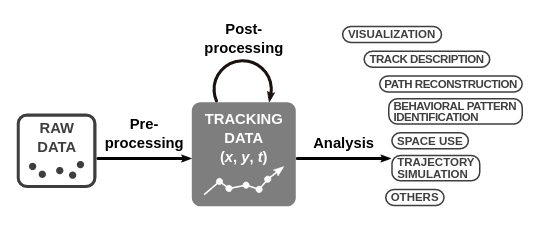
\includegraphics[width=0.95\linewidth]{img/joo2020} 

}

\caption{Figure from Joo et al 2020}\label{fig:unnamed-chunk-1}
\end{figure}
\end{frame}

\begin{frame}[fragile]
\begin{block}{Packages that we will use}
\phantomsection\label{packages-that-we-will-use}
\begin{itemize}
\item
  We will mainly use the \texttt{amt} package, but also occasionally
  other packages for movement analysis.
\item
  See also \texttt{required\_packages.R} for a list of all packages that
  we need and to get the latest version of all packages.
\end{itemize}
\end{block}
\end{frame}

\begin{frame}[fragile]{Some conventions in R}
\phantomsection\label{some-conventions-in-r}
\begin{itemize}
\tightlist
\item
  \texttt{\%\textgreater{}\%} or \texttt{\textbar{}\textgreater{}}:
  Pipes the output of one function to a next function. We will discuss
  this further later on.
\item
  \texttt{::} to access a name space form a package.
\item
  use of `a`.
\item
  \texttt{.} means this directory
\item
  \texttt{..} refers to the parent directory
\item
  \texttt{data.frame} or \texttt{tibble}?
\end{itemize}
\end{frame}

\begin{frame}[fragile]
\begin{itemize}
\tightlist
\item
  We often use \texttt{here::here("path\ to\ a\ file")}, when reading in
  a file.
\item
  The first \texttt{here} calls the function \texttt{here()} from the
  package \texttt{here}.
\item
  The function \texttt{here()} dynamically creates the absolute path to
  the project root.
\end{itemize}

\begin{Shaded}
\begin{Highlighting}[]
\NormalTok{here}\SpecialCharTok{::}\FunctionTok{here}\NormalTok{()}
\end{Highlighting}
\end{Shaded}

\begin{verbatim}
[1] "/Users/jsigner/git/movement_workshop"
\end{verbatim}

This means, that we save all our data in the root directory data (even
though my scripts are in different sub directories).
\end{frame}

\begin{frame}[fragile]
\begin{block}{Brackets (\texttt{(}, \texttt{{[}}, \texttt{\{})}
\phantomsection\label{brackets}
\begin{itemize}
\tightlist
\item
  round brackets or parentheses (\texttt{(}) usually indicate functions
  or are used in arithmetic calculations.
\end{itemize}

\begin{Shaded}
\begin{Highlighting}[]
\FunctionTok{sqrt}\NormalTok{(}\DecValTok{3}\NormalTok{)}
\end{Highlighting}
\end{Shaded}

\begin{verbatim}
[1] 1.732051
\end{verbatim}

or

\begin{Shaded}
\begin{Highlighting}[]
\DecValTok{2} \SpecialCharTok{*}\NormalTok{ (}\DecValTok{3} \SpecialCharTok{+} \DecValTok{1}\NormalTok{)}
\end{Highlighting}
\end{Shaded}

\begin{verbatim}
[1] 8
\end{verbatim}
\end{block}
\end{frame}

\begin{frame}[fragile]
\begin{itemize}
\tightlist
\item
  square brackets (\texttt{{[}}, \texttt{{[}{[}}) are used to subset
  data structures.
\end{itemize}

\begin{Shaded}
\begin{Highlighting}[]
\NormalTok{letters[}\DecValTok{1}\SpecialCharTok{:}\DecValTok{3}\NormalTok{]}
\end{Highlighting}
\end{Shaded}

\begin{verbatim}
[1] "a" "b" "c"
\end{verbatim}

or

\begin{Shaded}
\begin{Highlighting}[]
\FunctionTok{head}\NormalTok{(iris[[}\StringTok{"Species"}\NormalTok{]])}
\end{Highlighting}
\end{Shaded}

\begin{verbatim}
[1] setosa setosa setosa setosa setosa setosa
Levels: setosa versicolor virginica
\end{verbatim}
\end{frame}

\begin{frame}[fragile]
\begin{itemize}
\tightlist
\item
  curly brackets or braces (\texttt{\{}) are used to form code blocks
  (e.g., inside a function or control structure).
\end{itemize}

\begin{Shaded}
\begin{Highlighting}[]
\ControlFlowTok{for}\NormalTok{ (i }\ControlFlowTok{in} \DecValTok{1}\SpecialCharTok{:}\DecValTok{10}\NormalTok{) \{}
\NormalTok{  i}\SpecialCharTok{\^{}}\DecValTok{2}
\NormalTok{\} }
\end{Highlighting}
\end{Shaded}
\end{frame}

\begin{frame}[fragile]
\begin{block}{Functions}
\phantomsection\label{functions}
\begin{itemize}
\tightlist
\item
  Functions \emph{do} something. For example function \texttt{sqrt()}
  takes the square root for a number.
\item
  It is easy to recognize functions, because they usually have a name
  (e.g., \texttt{sqrt}) followed by round brackets \texttt{()}.
\item
  Within these round brackets arguments are passed to a function. This
  arguments can be named or unnamed (as long as they are in the correct
  order).
\end{itemize}
\end{block}
\end{frame}

\begin{frame}{Recommended setup}
\phantomsection\label{recommended-setup}
\begin{itemize}
\item
  We would recommend to download the whole repository from GitHub
  (\url{https://github.com/jmsigner/movement_workshop_spring2025})\footnote<.->{If
    you are familiar with git, feel free to clone the repository}.
\item
  Then use the RStudio project (together with RStudio).
\item
  Following these guides, you should have all paths correct.
\end{itemize}
\end{frame}

\begin{frame}{Geographic data in brief}
\phantomsection\label{geographic-data-in-brief}
\begin{itemize}
\item
  Movement data is inherently spatial.
\item
  Thus we will have to deal with tools to work with spatial data (R has
  a rich set of tools to deal with spatial data;
  e.g.~\url{https://geocompr.robinlovelace.net/}).
\item
  We will work frequently with raster data (spatial covariates) and
  possibly with vector data (i.e., home ranges).
\item
  One of the challenges is to ensure that both -- tracking data and
  covariates -- have a matching coordinate reference system (CRS).
\end{itemize}
\end{frame}

\begin{frame}
\begin{itemize}
\tightlist
\item
  The CRS defines the reference system that is being used to explicitly
  reference a feature in space.
\item
  There are two classes of CRS: \textbf{geographic} (e.g., WGS84) and
  \textbf{projected} (e.g., UTM) CRS.
\item
  Projected CRS flatten the three dimensional data to the a
  two-dimensional plane (and introduce some distortion). \pause
\item
  CRS are often referred to with their EPSG\footnote<.->{EPSG stands for
    European Petrol Survey Group, who came up with the system.} code.
\item
  EPSG codes are four to five digits number that refer to different CRS.
  See for example www.epsg.io. \pause
\item
  Which CRS is best to use? It depends on the range of the study
  species. I usually prefer projected CRS, because their units are
  meters and not degrees.
\end{itemize}
\end{frame}

\begin{frame}{Data}
\phantomsection\label{data}
\begin{block}{Movement data}
\phantomsection\label{movement-data}
\begin{itemize}
\tightlist
\item
  Often times the data we receive is just a time series of coordinates
  (longitude, latitude and time stamp).
\item
  Depending on the sensors we use, other (meta) information may also be
  stored (this could include temperature, coordinates in a different
  {[}projected{]} CRS, \ldots).
\end{itemize}

\begin{figure}

{\centering 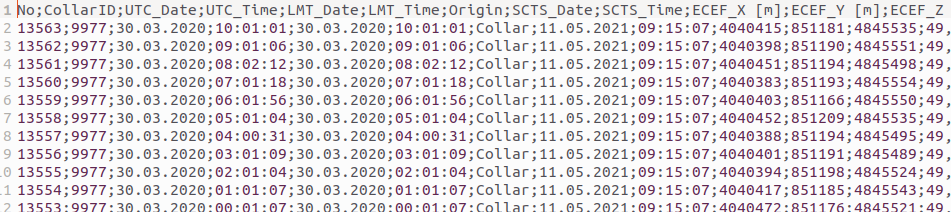
\includegraphics[width=0.85\linewidth]{../img/relocs} 

}

\end{figure}
\end{block}
\end{frame}

\begin{frame}
\begin{block}{Environmental covariates}
\phantomsection\label{environmental-covariates}
\begin{itemize}
\tightlist
\item
  Vector layers (e.g., road networks, rivers, protected areas)
\item
  Raster layers (e.g., land use, remotely sensed data such as NDVI,
  climatic variables)
\end{itemize}
\end{block}
\end{frame}

\begin{frame}[fragile]{Tracks and bursts: the basic building block}
\phantomsection\label{tracks-and-bursts-the-basic-building-block}
\begin{itemize}
\item
  For movement data, we usually read a text file into R (\texttt{.csv},
  \texttt{.txt}, \ldots) as a data frame and then create a
  analysis-specific object.
\item
  When working with the \texttt{amt} package the function
  \texttt{make\_track()} takes a sequence of coordinates (with or
  without timestamps) and creates a track. Note, at this point multiple
  individuals can be mixed and sampling rates can be heterogeneous.
\end{itemize}
\end{frame}

\begin{frame}
\begin{itemize}
\tightlist
\item
  \textbf{Bursts} can be created from tracks.
\item
  A burst is a sequence of (re)locations from the \textbf{same}
  individual at \textbf{equal} time intervals (with some tolerance).
\end{itemize}

\begin{figure}

{\centering 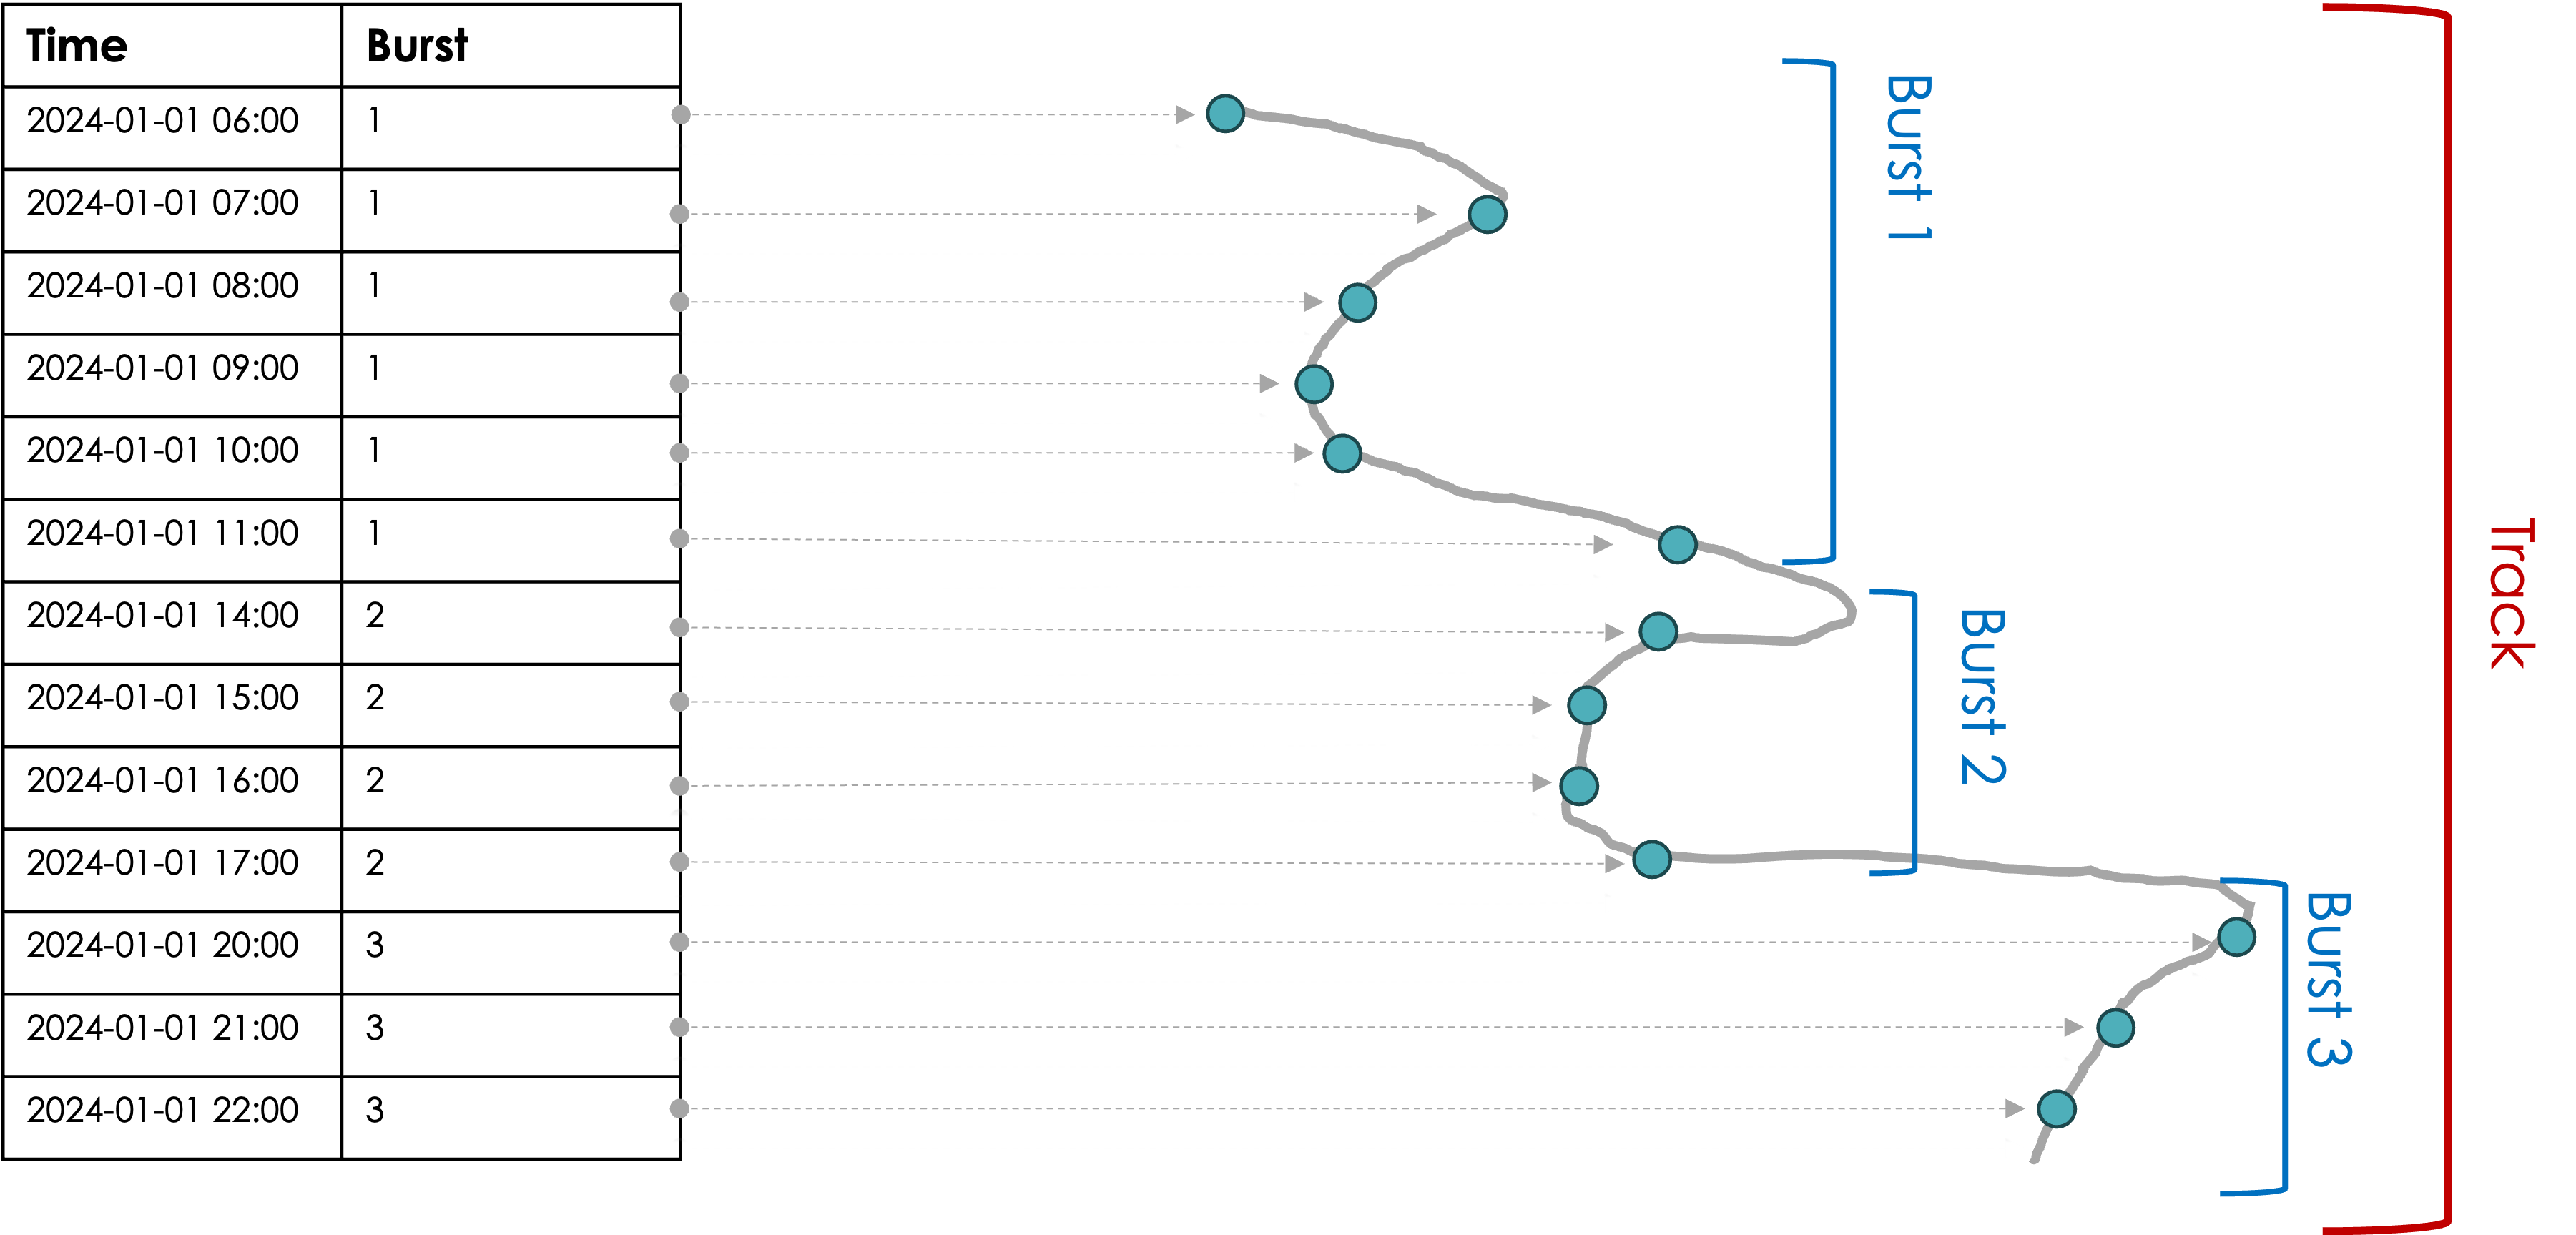
\includegraphics[width=0.85\linewidth]{../img/track_burst} 

}

\end{figure}
\end{frame}

\begin{frame}[fragile]{Sampling rates, and resampling}
\phantomsection\label{sampling-rates-and-resampling}
\begin{itemize}
\tightlist
\item
  The function \texttt{summarize\_sampling\_rate()} takes a track as
  input and gives a summary of the sampling rate.
\item
  If there are multiple animals present, there is also the function
  \texttt{summarize\_sampling\_rate\_many()}, which will do the same
  thing, but for many animals.
\end{itemize}
\end{frame}

\begin{frame}[fragile]
\begin{itemize}
\tightlist
\item
  Once a suitable sampling rate is determined, the function
  \texttt{track\_resample()} can be used to take a relocation every
  predefined time interval (e.g., 30 minutes, 2 hours, \ldots) within a
  tolerance.
\item
  The result of \texttt{track\_resample()} is again a track with one
  additional column called \texttt{burst\_}.
\end{itemize}
\end{frame}

\begin{frame}
If you have gaps and/or different sampling rates, interpolation with
continuous time movement models may be an option.

\begin{figure}

{\centering 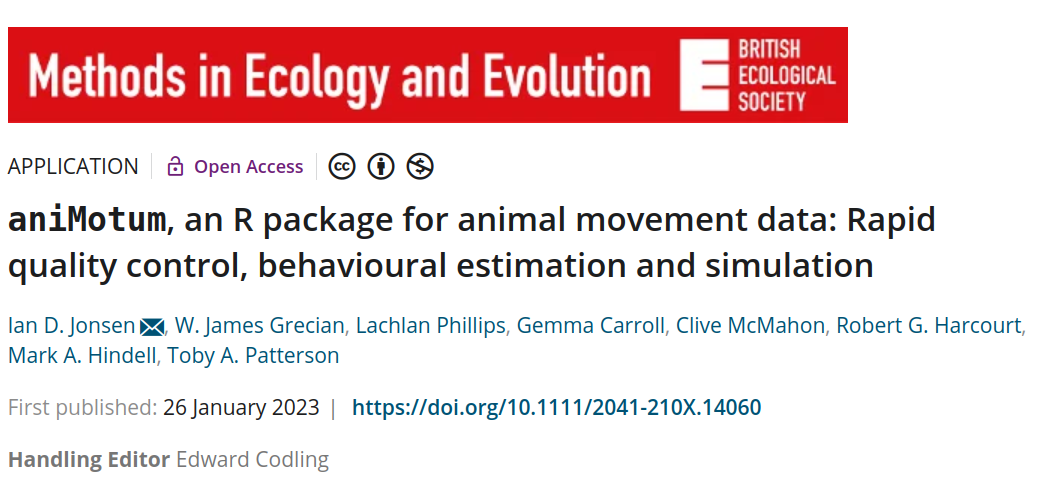
\includegraphics[width=0.85\linewidth]{../img/jonsen2023_mee} 

}

\end{figure}
\end{frame}

\begin{frame}
An more specifically for Step-Selection Functions

\begin{figure}

{\centering 
\includegraphics[width=0.85\linewidth]{../img/Hofmann2024} 

}

\end{figure}
\end{frame}

\begin{frame}{Movement characteristics (\texttt{sl\_}, \texttt{ta\_})}
\phantomsection\label{movement-characteristics-sl_-ta_}
Tracks are still \emph{just} the points as they were collected. If we
want to get insights, we have can look at different characteristics of
steps (i.e., two consecutive relocations).

This include:

\begin{itemize}
\tightlist
\item
  step length
\item
  turn angle
\item
  speed
\item
  Net squared displacement
\end{itemize}

Note, unless you take care of different instances or bursts, they are
ignored.
\end{frame}

\begin{frame}[fragile]{Net Squared displacement (NSD)}
\phantomsection\label{net-squared-displacement-nsd}
\begin{itemize}
\tightlist
\item
  The NSD is the squared distance between the first relocation of a
  track and the every relocation that follows.
\item
  Bunnefeld et al.~2011 described different forms of the NSD that
  resemble different migratory behaviors.
\item
  The different models can fit to the data (e.g., using nonlinear least
  square with the function \texttt{nls()} in R).
\end{itemize}
\end{frame}

\begin{frame}
\begin{figure}

{\centering 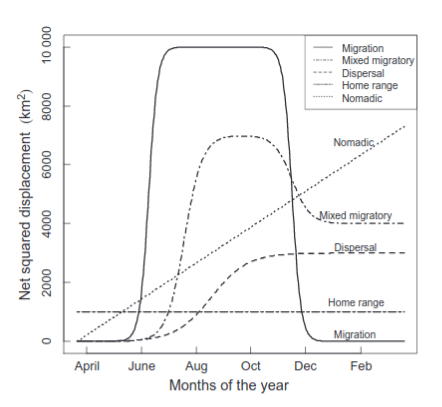
\includegraphics[width=0.6\linewidth]{img/nsd} 

}

\caption{Figure taken from Bunnefeld et al. 2011}\label{fig:unnamed-chunk-12}
\end{figure}
\end{frame}

\begin{frame}[fragile]{Time of the day}
\phantomsection\label{time-of-the-day}
\begin{itemize}
\tightlist
\item
  Time of day can be annotated to steps with the function
  \texttt{amt::time\_of\_day()}. This will add an additional column to
  the data frame of steps \texttt{tod\_end} or \texttt{tod\_start}
  depending on the argument \texttt{when}.
\item
  If the data is of sufficient temporal resolution, it is also possible
  to annotate twilight (dawn and dusk).
\end{itemize}
\end{frame}

\begin{frame}[fragile]{Steps}
\phantomsection\label{steps}
We can start to create a \texttt{steps}-representation.

\begin{center}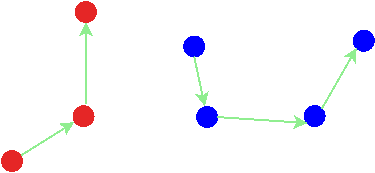
\includegraphics[width=0.5\linewidth]{img/steps} \end{center}

This can be achieved with the function \texttt{amt::steps()}. If we
resampled the data previously, we can even use
\texttt{amt::steps\_by\_burst()}.
\end{frame}

\begin{frame}
\begin{center}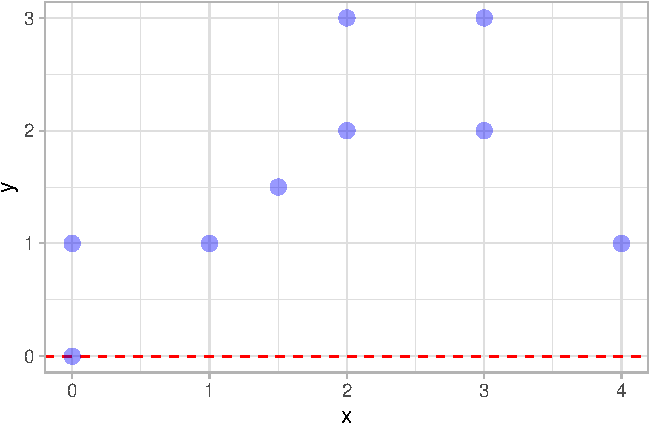
\includegraphics[width=0.85\linewidth]{01a_lecture_files/figure-beamer/unnamed-chunk-14-1} \end{center}
\end{frame}

\begin{frame}
\begin{center}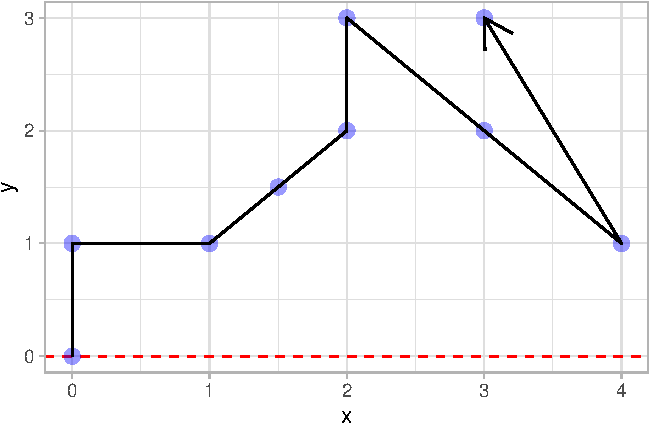
\includegraphics[width=0.85\linewidth]{01a_lecture_files/figure-beamer/unnamed-chunk-15-1} \end{center}
\end{frame}

\begin{frame}
\begin{center}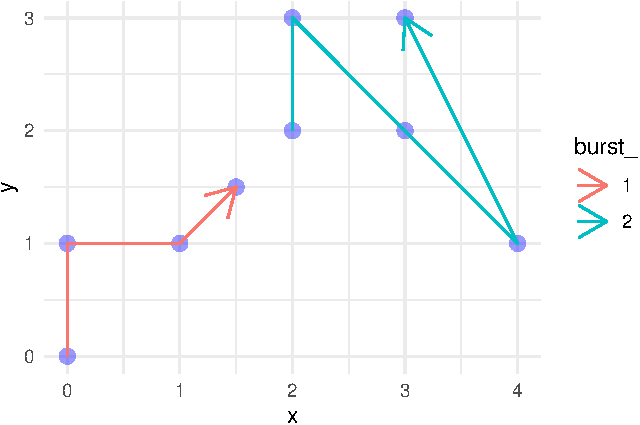
\includegraphics[width=0.85\linewidth]{01a_lecture_files/figure-beamer/unnamed-chunk-16-1} \end{center}
\end{frame}

\begin{frame}
This automatically calculates several step attributes:

\begin{itemize}
\tightlist
\item
  Start and end point
\item
  Step length
\item
  Absolute and relative turn angles
\item
  Duration
\end{itemize}

This allows already calculate some step characteristics. It becomes even
more informative, if we pair this for example with the whether a step
was in the night, day or twilight.
\end{frame}

\begin{frame}{Example}
\phantomsection\label{example}
Remington Moll observed a (rare) long distance dispersal for White Tail
deer\footnote<.->{Moll et. al Ecology and Evolution;
  \url{https://onlinelibrary.wiley.com/doi/full/10.1002/ece3.7354}.} and
looked at the turn angle and step distribution for day and night.

\begin{center}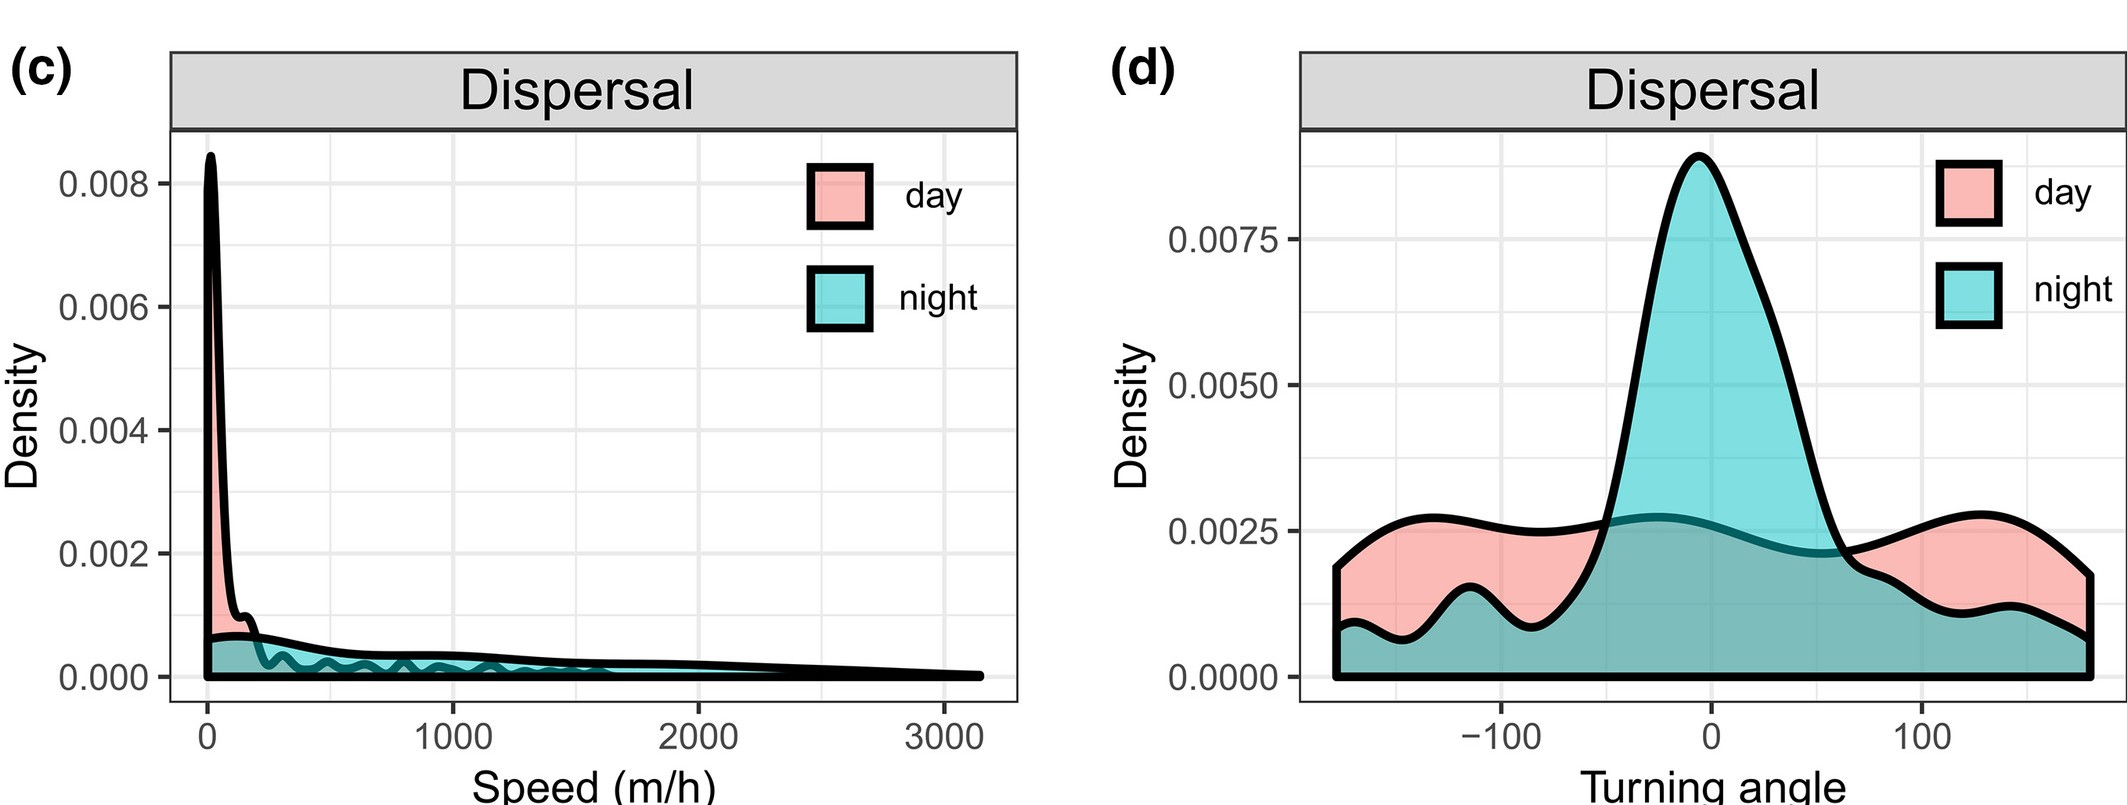
\includegraphics[width=0.85\linewidth]{img/moll3_part} \end{center}
\end{frame}

\begin{frame}{Data sets that we use}
\phantomsection\label{data-sets-that-we-use}
\begin{itemize}
\tightlist
\item
  We will use several data sets during this course including a data set
  on fishers, elephants and deer.
\item
  Feel free to use your own data during the exercises, we are happy to
  help to get it into shape.
\item
  For the R walkthrough we often simulate data. We believe if understand
  how data is generated it is much easier to understand how a specific
  method works.
\end{itemize}
\end{frame}


\end{document}
